\section{Hardware Design}

FANS is composed of various hardware components to perform its desired functionality.

\subsection{Raspberry Pi SenseHat}

The Raspberry Pi SenseHat is responsible for providing the temperature data readings collected by the smoke detection
system. This component was chosen because it's readily available and also has a large number of tutorials available for
integrating it into systems \cite{sensehat}. A diagram is not shown as the SenseHat is self-contained and can simply be
directly place on top of the Raspberry Pi 4, connected via the GPIO pin headers.

\subsection{MQ2 Smoke Sensor}

The MQ2 Smoke Sensor is a critical component in the FANS project, chosen for its capability to detect a wide range of
gases that occur, including smoke, which is essential for early fire detection. It operates at 5V and outputs an analog
signal that varies with the concentration of detected gases. The sensor's sensitivity to smoke enables the system to
promptly identify fire hazards, triggering alerts and activating safety measures. Its analog output necessitates an
analog-to-digital converter (ADC) when used with a Raspberry Pi, ensuring accurate detection levels are communicated to
the system for processing and response.

\begin{figure}[H]
    \centering
    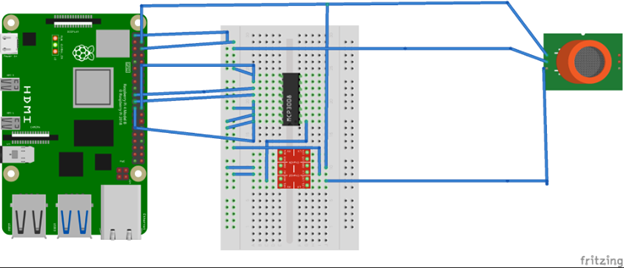
\includegraphics[width=3in]{../assets/schematics/MQ2SensorBB.png}
    \caption{Bread board configuration of the smoke sensor.}
\end{figure}

\begin{figure}[H]
    \centering
    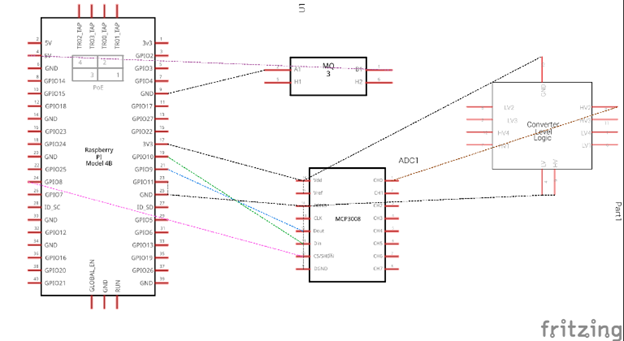
\includegraphics[width=3in]{../assets/schematics/MQ2SensorSchematic.png}
    \caption{Schematic of the smoke sensor circuit.}
\end{figure}

\subsection{LCD Display}

The project incorporates a 16x2 character LCD Display for real-time monitoring, utilizing the I2C communication
protocol for easy interfacing with the Raspberry Pi . This display operates on either 5V or 3.3V and is used to flash
in an emergency to indicate as smoke levels and temperature rise directly to the user. The choice of an LCD display
ensures that information about the environmental condition is immediately accessible, providing a quick overview
without needing to access the system digitally.

\begin{figure}[H]
    \centering
    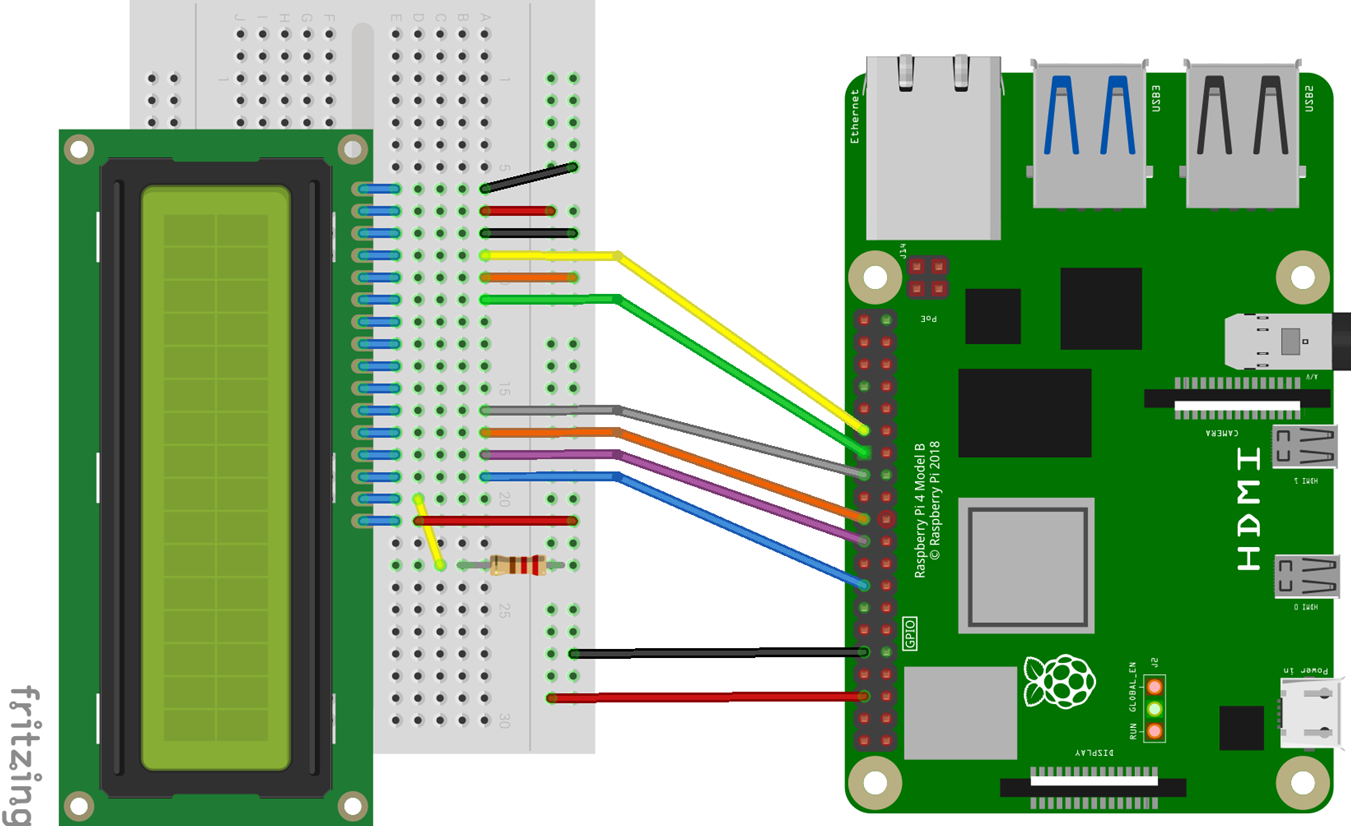
\includegraphics[width=3in]{../assets/schematics/LCDBB.png}
    \caption{Bread board configuration of the LCD display.}
\end{figure}

\begin{figure}[H]
    \centering
    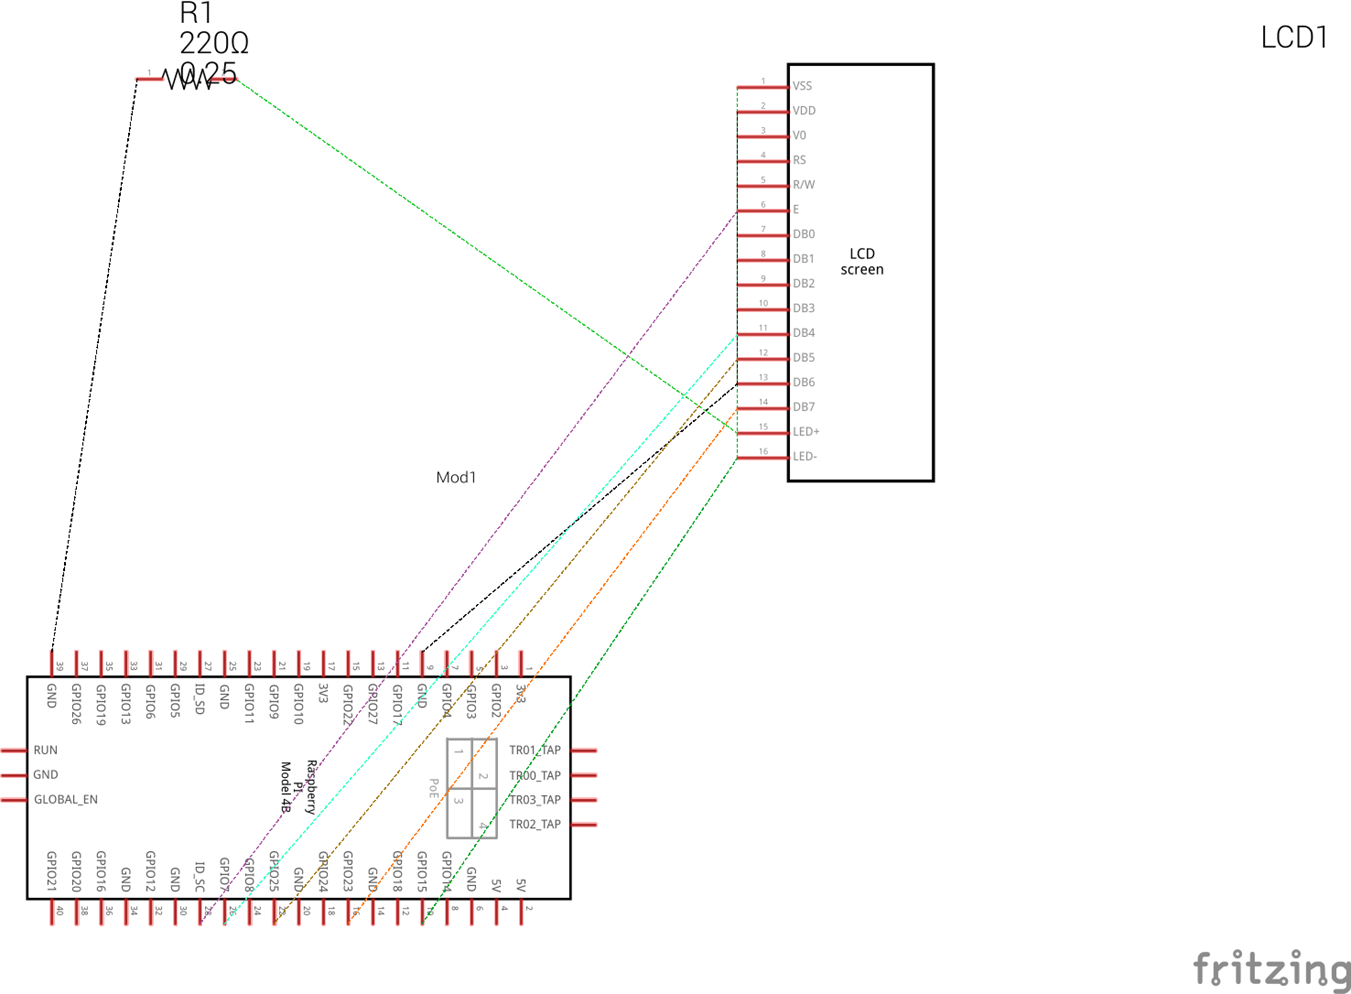
\includegraphics[width=3in]{../assets/schematics/LCDSchema.png}
    \caption{Schematic of the LCD display circuit.}
\end{figure}

\subsection{Piezoelectric Buzzer}

The inclusion of a simple piezoelectric buzzer in the system design offers an effective way to generate audible alerts
when smoke or high temperatures are detected. Operating between 3.3V to 5V and controlled via a GPIO pin, the buzzer
can produce a range of tones, making it a versatile component for different alert types. It ensures that the system can
attract attention through sound, complementing visual alerts and enhancing the overall effectiveness of the fire
detection system.

\begin{figure}[H]
    \centering
    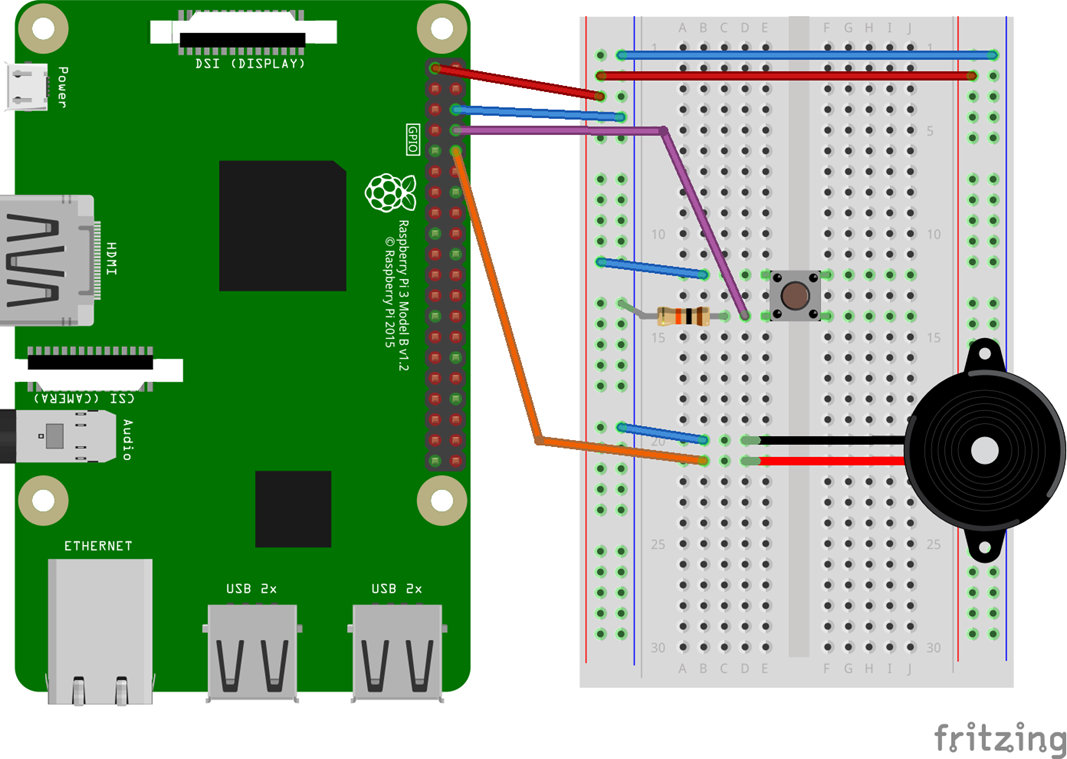
\includegraphics[width=3in]{../assets/schematics/BuzzerBB.png}
    \caption{Bread board configuration of the piezoelectric buzzer.}
\end{figure}

\begin{figure}[H]
    \centering
    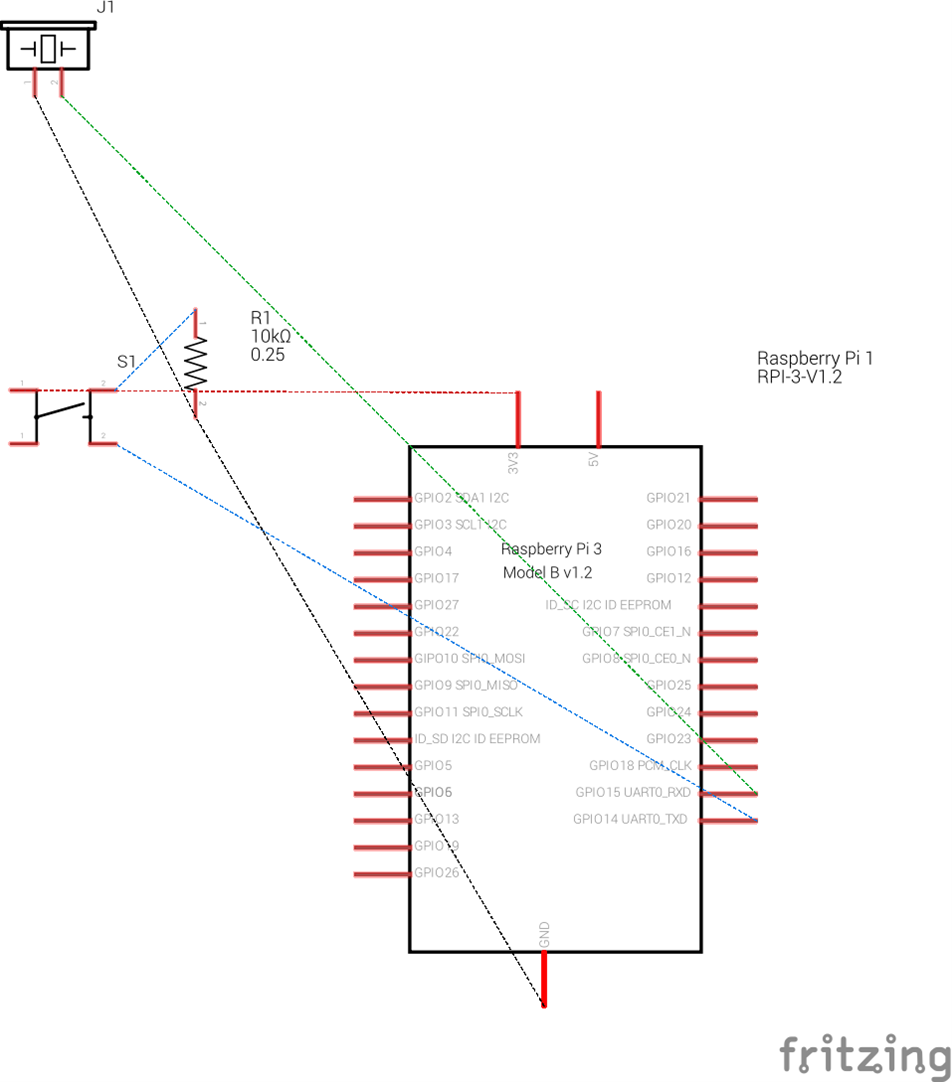
\includegraphics[width=3in]{../assets/schematics/BuzzerSchema.png}
    \caption{Schematic of the piezoelectric buzzer circuit.}
\end{figure}

The following schematics show the connections between the piezoelectric buzzer and the Raspberry Pi Pico. There is no
Fritzing footprint for the Pi Pico, so the Raspberry Pi 4 is used as a placeholder.

\begin{figure}[H]
    \centering
    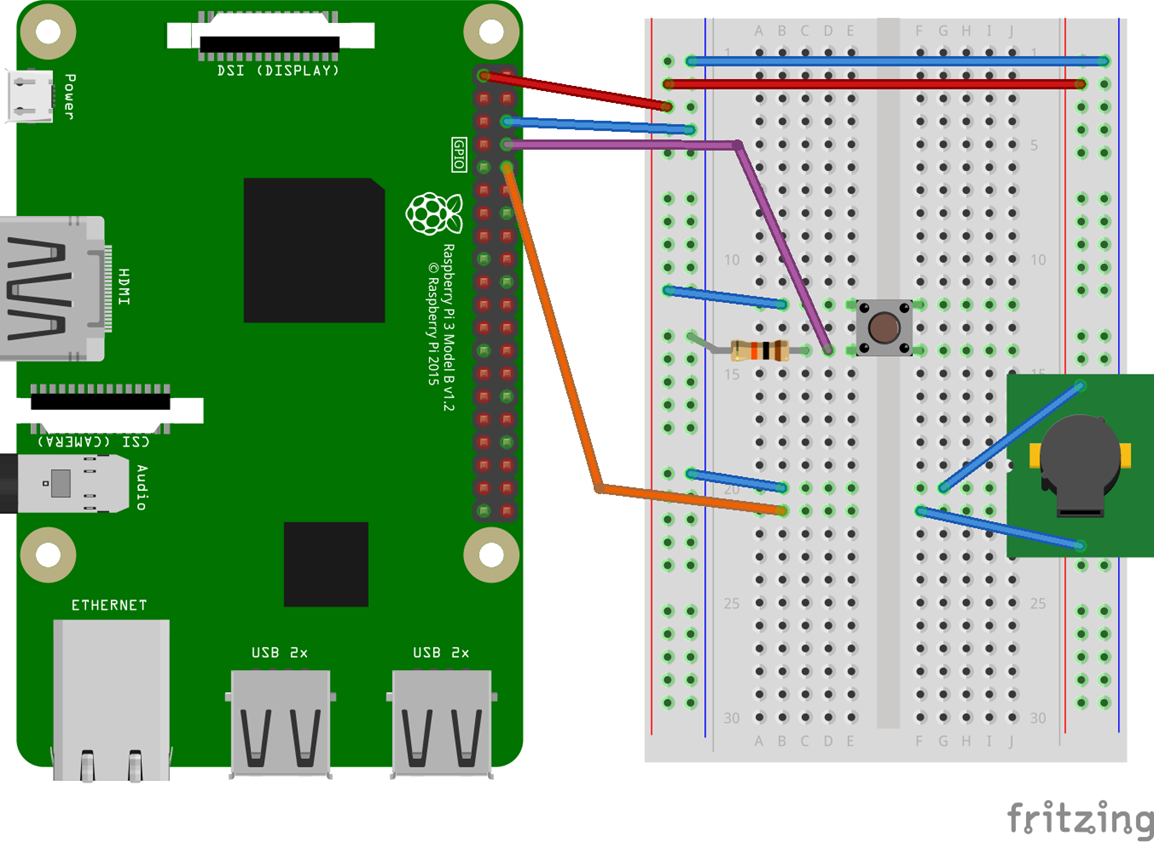
\includegraphics[width=3in]{../assets/schematics/AudiohatBB.png}
    \caption{Bread board configuration of the piezoelectric buzzer with the Pi Pico.}
\end{figure}

\begin{figure}[H]
    \centering
    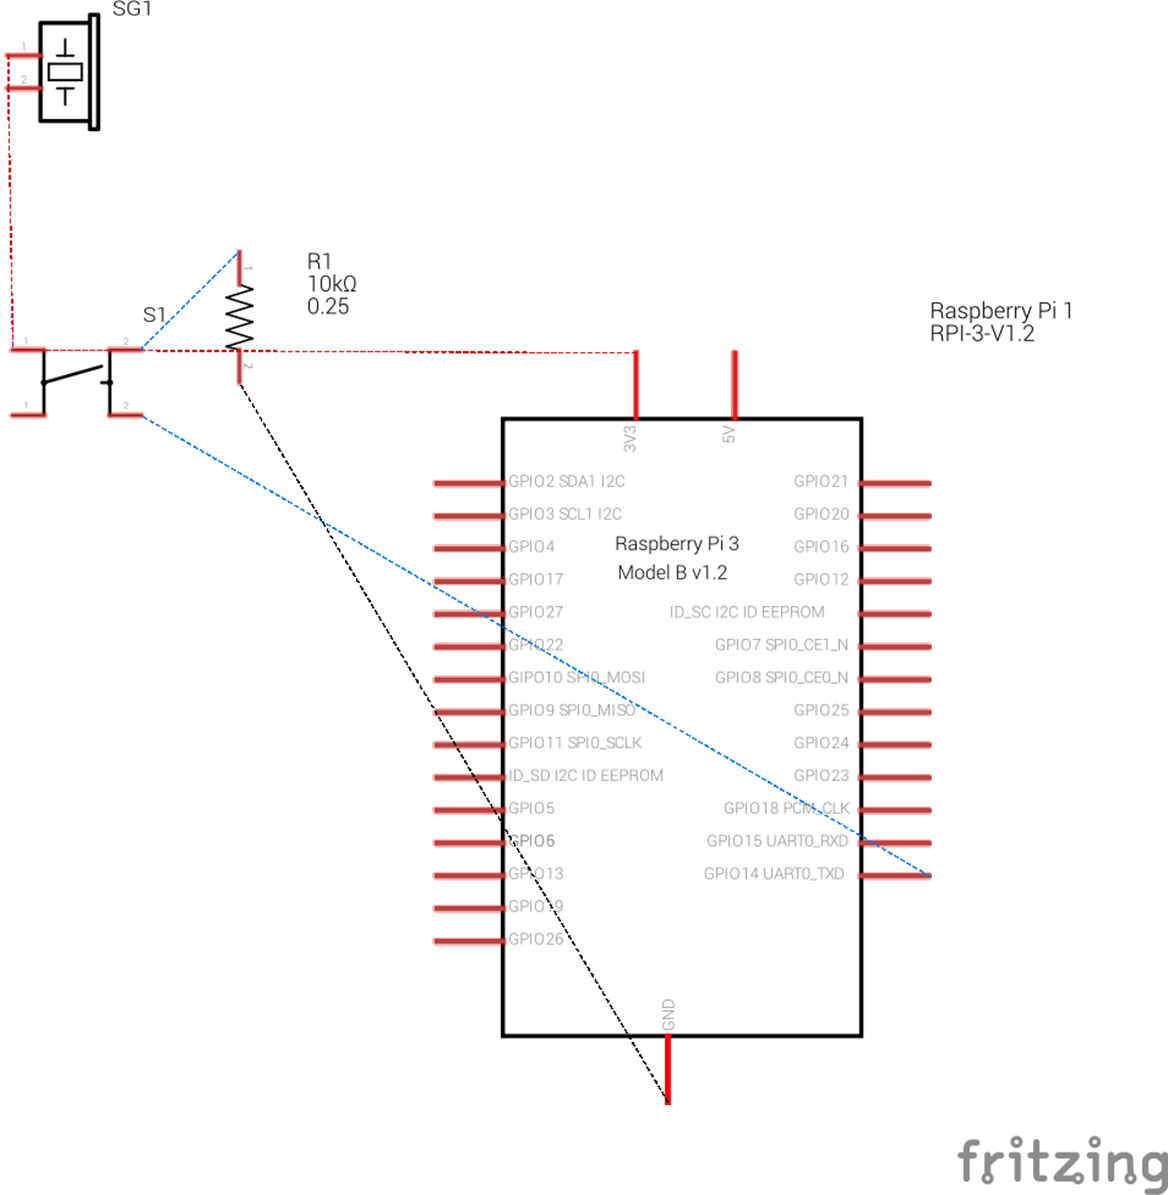
\includegraphics[width=3in]{../assets/schematics/AudiohatSchema.png}
    \caption{Schematic of the piezoelectric buzzer circuit connected to the Pi Pico.}
\end{figure}
